\section{The Arm TrustZone Solution}
Arm released TrustZone in 2004 for their ``application capable'' cores, and only as recently as 2016 did they extend this technology to their cores designed for microcontrollers \cite{Pinto2019}. When evaluating how Arm’s TrustZone works, we must remember several important distinctions. Firstly, the Arm specifications include several different architectures with several different states. Each Arm architecture and state combination may operate slightly differently in regard to how TrustZone is implemented. This thesis will only consider the ARMv8-A architecture running in the AArch64 state. Secondly, because Arm Limited licenses their cores to hardware manufacturers, \glspl{soc} and platforms may choose to implement security in many ways, and with much more flexibility than in Intel platforms. For simplicity’s sake, this paper will only cover firmware solutions for TrustZone implementations provided by Linaro's open source projects \gls{tfa} and \gls{optee}.
 
Arm \gls{soc} processors create a more absolute separation between the concepts of ``secure'' and ``normal or insecure'' operation than Intel \gls{sgx}. At its highest level this is accomplished using the \gls{scr} ``Non-Secure bit'' (NS) with 1 meaning non-secure and 0 meaning secure. This is perhaps the most fundamental element that separates Arm's two security worlds. Digging a bit deeper, this separation of worlds is accomplished using four separate primitives: one on the bus, one on the \gls{soc} core, one as part of the memory infrastructure, and finally one as part of the debug infrastructure.

Firstly, the bus interface, called the \gls{amba} \gls{axi}, partitions all of the \gls{soc}’s hardware and software resources by taking advantage of a set of bits. Hardware logic present in this ``TrustZone-enabled AMBA3 AXI  bus fabric'' \cite{ArmBuildingSS} ensures that no ``Secure World'' resources can be accessed by ``Normal World'' components. These bits include AWPROT for write transactions and ARPROT for read transactions where like the NS bit low is Secure and high is Non-secure. 

Secondly, \gls{soc}s which include cores like the ARMv8-A, implement extensions which enable a single physical processor core to safely and efficiently execute code from both the Normal World and the Secure World in a time-sliced fashion \cite{TrustZoneExplained}. The value of the Non-Secure bit is read from the \gls{scr} and passed along down the bus to the memory controller and peripherals. A new instruction, the \gls{smc}, is added which allows the core to switch between the secure and normal modes. We will discuss the secure monitor firmware which is responsible for handling these interrupts in the next section.

Thirdly, the memory infrastructure includes security features like \gls{tzasc} and \gls{tzma} \cite{TrustZoneExplained}. The \gls{tzasc} allows for configuration of the secure and normal world memory regions. It does so by partitioning DRAM into areas which have secure world access and those regions which have normal world access. This process can only be done from the secure world. The \gls{tzma} serves a similar function for any off-chip memory such as an off-chip ROM. The way in which this memory partitioning happens is based on the specific SoC implementing TrustZone. SoC manufacturers can provide robust or simple partitioning and it is important to understand the implementation of your specific SoC's memory controller to properly understand how TrustZone has been implemented.

Lastly, the security-aware debug infrastructure controls debug access to the Secure World. This includes ``secure privileged invasive (JTAG) debug, secure privileged non-invasive (trace) debug, secure user invasive debug, and secure user non-invasive debug'' \cite{ArmBuildingSS}. By using two different signals into the core along with two different bits in a secure register, the core can report either invasive or non-invasive debug info. In this way, the core is able to debug either the normal world only, or it can debug both the secure and normal worlds together. These four primitives provide a framework or scaffolding on which to build a platform capable of secure computation.

In the next section we discuss the firmware that will implement a \gls{tee} using TrustZone's features. First, we will point out a potentially confusing difference between how Intel and Arm create privilege levels. Unlike Intel platforms which refer to their privilege levels as rings, Arm uses ``Exception Levels'' EL0 through EL3 \cite{armfundv8A}. Here EL3 is the highest, most privileged level where as EL0 is the lowest and least privileged level. Much like with the x86 architecture, exceptions like data aborts, pre-fetch aborts, and other interrupts can be taken from the level at which they occur to the same or any higher privileged level, but not a level which has less privileges. So, for example, an interrupt occurring in the OS kernel (EL1) can be handled in the kernel or in the secure monitor (EL3), but not in the lower privileged application level (EL0). Practically speaking this means that the user applications running on a system which has not been compromised will not have access to kernel or lower exceptions. Another common confusion point between Arm and Intel is that Intel's ``ring 0'' is the highest privilege level while Arm's ``EL0'' is the lowest privilege level.

\renewcommand{\arraystretch}{2.5}
\begin{table}[t]
\centering
\begin{tabular}{|l|l|l|}
\hline
\textbf{Privilege Level} & \textbf{Description} & \textbf{Implementation}                                          \\ \hline
EL-0 & Application Privilege Level & Supported by CPU architecture                                                   \\ \hline
EL-1 & Kernel Privilege Level & Supported by CPU architecture                                                   \\ \hline
EL-2 & \makecell[l]{Virtualization Privilege Level \\ (Optional)} & Supported by CPU architecture                                                   \\ \hline
EL-3 & Secure Privilege Level & \makecell[l]{Supported by CPU architecture \\ or a dedicated embedded \\ security processor} \\ \hline
\end{tabular}
\caption{Arm Privilege Level Mapping}
\label{table:arm_priv_lev_map}
\end{table}


See Figure \ref{table:arm_priv_lev_map} for a complete list of privilege levels, their description, and how they might be implemented in an ARMv8-A system. Each exception level manages its own page tables and control registers with the exception of EL0 which is managed by EL1 \cite{armfundv8A}. This is a common practice across architectures where the kernel level mode controls the page table for the applications running on top of it. As we will see, this division is taken advantage of by the ARMv8-A architecture to enable the separation of memory accesses between the Secure World and the Normal World.

\section{Arm Trusted Firmware}
Since 2013, Arm, in cooperation with several other industry leaders, has provided \glsreset{tfa}\gls{tfa} as an open source reference implementation of the firmware required to develop Secure World software for A-Class devices (including ARMv8-A). \gls{tfa} provides many features including secure device initialization, modular boot flow, trusted boot, and the secure monitor that allows switching between the Normal World and the Secure World. It should be noted that all of this code and documentation is freely available online \cite{urlTrustedFirmware}. The Trusted Firmware Project is a `not for profit' open source project hosted by Linaro Limited (``Linaro'').

Arm Trusted Firmware uses the scaffolding provided by the A-Class devices to implement the key aspects of TrustZone, namely Trusted Boot and the Secure Monitor. There are currently over 30 platforms supported by Trusted Firmware and because the code is open source (BSD 3-clause), porting new platforms can be done by following many of the existing open source examples. Before we explore Arm Trusted Firmware, we must first understand how an Arm platform can be initialized in a secure state, specifically using \gls{tbb}. \gls{tbb} is based on two standards, the Arm Trusted Base System Architecture (TBSA) \cite{Edition2018} and the Arm Trusted Board Boot Requirements (TBBR) \cite{ArmTrustedBoot}. Both of these specifications are client-based solutions and it is likely that server based solutions are in development internally at Arm.

\begin{figure}[ht]
\centering
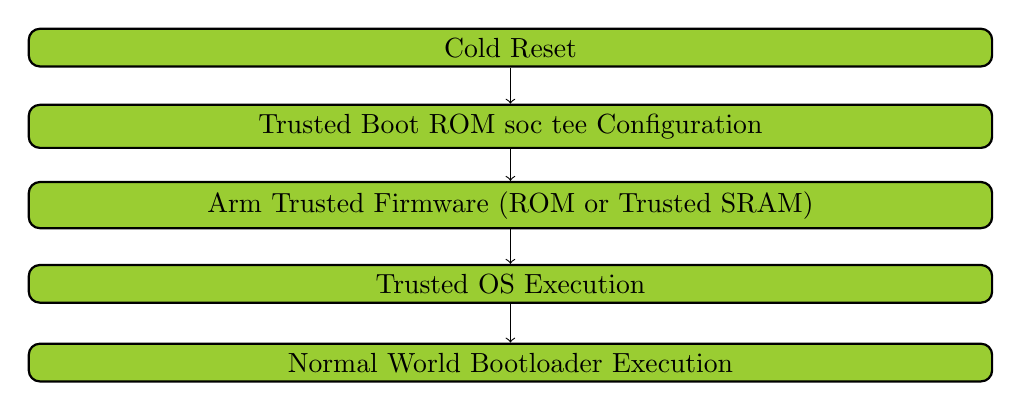
\begin{tikzpicture}[
    block/.style ={rectangle, draw=black, thick, fill=YellowGreen,
          text width=12cm, text centered, rounded corners},
    line/.style ={draw, ->}
]

\node[block] (s1) at (0,0) {Cold Reset};
\node[block, below of = s1] (s3) {Trusted Boot ROM \gls{soc} \gls{tee} Configuration};
\node[block, below of = s3] (s5) {Arm Trusted Firmware (ROM or Trusted SRAM)};
\node[block, below of = s5] (s10) {Trusted OS Execution};
\node[block, below of = s10] (s15) {Normal World Bootloader Execution};

\path [line] (s1) -- (s3);
\path [line] (s3) -- (s5);
\path [line] (s5) -- (s10);
\path [line] (s10) -- (s15);

\end{tikzpicture}

\caption[Arm's Trusted Board Boot]{\textbf{A significantly simplified boot flow for setting up a secure \gls{rot} on an Arm system running Trusted Firmware.} Here we see the boot flow from a cold reset all the way to the Normal World bootloader which may load any untrusted OS kernel.}
\label{fig:tbb-flow}
\end{figure}

As soon as the SoC comes out of power-on-reset, execution happens in integrity protected memory like on-chip Boot ROM or Trusted SRAM. At this stage we have access to a \gls{rotpk} located in one of the \gls{soc}'s \gls{otp} Efuse registers. These keys are usually SHA-256 and the Efuse is burned by the manufacturer to ensure the integrity of the keys. This secure ROM firmware code is often called the Bootloader Stage 1 or BL1, and it is responsible for checking the validity of the \gls{rotpk}. Using this key, BL1 can verify the hash of the next bootloader stage (BL2). The code in BL1 is the only code that must run in EL3, minimizing the amount of initialization code that must run at this critical privilege level.

Once in BL2, the code is executing in Secure World EL2 and the firmware can use the \gls{rotpk} to extract the Trusted World \gls{rotpk} and the Normal World \gls{rotpk}, which are used in turn to validate the Secure World Trusted OS hash as well as the Normal World Untrusted OS hash. All of these keys and hashes are included as extensions to the x.509 standard format, however there is no need for a valid Certified Authority (CA) certificate, as we are verifying the contents of the certificates and not the validity of a certificate issuer. BL2 also does some RAM initialization before it passes off to BL3 where the Secure Monitor is implemented.

This Secure Monitor runs in EL3 and is responsible for loading both the Secure OS as well as the Normal World bootloader (like U-Boot or some UEFI implementation). This Secure Monitor stays resident in memory during the life of the system and will manage the interactions between the Normal and Secure Worlds. All of these stages (BL1 - BL3) of \gls{tbb} are implemented by Arm's \glsreset{tfa}\gls{tfa} reference implementation.

\begin{figure}[ht]
\makebox[\textwidth][c]{\makebox[\linewidth]{
\begin{tikzpicture}[scale=0.8, transform shape,nodes={text width=3cm, align=center, minimum height=1cm}, small/.style={font=\small}]

% nodes
\node [draw,outer sep=0,inner sep=1] at (-9,10.5) {Generic Application};
\node [draw,outer sep=0,inner sep=1] (v1) at (-5,10.5) {App w/Security};
\node [draw,outer sep=0,inner sep=1] (v4) at (-9,8) {Scheduler};
\node [draw,outer sep=0,inner sep=1] (v2) at (-5,8) {TrustZone driver};
\node [draw] (v8) at (0.5,10.5) {Security Service};
\node [draw] (v7) at (4.5,10.5) {Standalone Application};
\node [draw] (v6) at (0.5,8) {Cross-world IPC manager};
\node [draw] (v5) at (4.5,8) {Scheduler};
\node [draw] (v3) at (0.5,6) {Secure Monitor};
\node [] at (-7,11.5) {Normal World};
\node [] at (2.5,11.5) {Secure World};
\node [] at (-7,9) {Kernel};
\node [] at (2.5,9) {Kernel};
\node [small] at (-12,9.75) {User};
\node [small] at (-12,9.25) {Privileged};
\node [small, minimum height=0] (v9) at (0.5,4) {EL3 Exception};

% edges
\draw[latex'-latex']  (v1) -- (v2);
\draw [latex'-latex'] (v2) |- (v3.170) node [near end, small, above, minimum height=0] {SMC};
\draw [-latex'] (v3) -| (v4);
\draw [latex'-] (v5) |- (v3);
\draw [latex'-latex'] (v8) -- (v6);
\draw [latex'-latex'] (v6) -- (v5);
\draw [latex'-latex'] (v3) -- (v6);

% fits
\begin{scope}[on background layer]
  \draw [dotted] (-11,12) rectangle (-3,5);
  \draw [dotted, fill=CornflowerBlue!10!white] (-1.5,12) rectangle (6.5,5);
\end{scope}
\draw [] (-10.75,9.25) rectangle (-3.25,7.25);
\draw [] (-1.25,9.25) rectangle (6.25,7.25);
\draw [dashed] (-13,9.5) -- (7,9.5);
\draw [-latex'] (v9) -- (v3);
\end{tikzpicture}
}

}\caption[Arm TrustZone Example of Normal and Secure World]{\textbf{Secure World implementation using ARM TrustZone.}
The \gls{soc} boots into the Secure World and a monitor is registered which acts as the interface between the ``secure'' and ``normal'' worlds. All EL3 exceptions are caught by the secure montior, and there is a special EL3 exception called a ``secure monitor call'' which is used to switch the processor between the two worlds. Figure recreated and modified from the original \cite{TeschkeSGX}.
\label{fig:tz-overview}}
\end{figure}

Once the Trusted Firmware has initialized the system in a secure state, we have initialized two worlds, the Trusted World and the Normal World. It is perhaps easiest to think about the interaction between these two worlds in much the same way we think about making calls from user mode into kernel mode in Linux systems. In Linux systems, we take advantage of system calls (syscall) to bridge a trust boundary between the kernel's concerns like interacting with a network card and the user application's concerns like displaying a web page. At no point in this interaction should the user application code have access to the network card's buffers, however the kernel is able to read and write these buffers and mediate the flow of data to/from the client application. This ``guarded'' flow of data is similar to how memory in the Secure World is kept separate from the Normal World using an instruction which generates an exception called a Secure Monitor Call (SMC).

\section{TrustZone Attestation}

Local \gls{attestation} using TrustZone is dependent on several \glspl{measurement} taken during the boot process. If the boot process is not secured then ``all bets are off'', and we cannot assure the integrity or confidentiality of the code or data inside the \gls{tee}. We will follow this boot flow step by step, and each step number is illustrated in Figure \ref{fig:tz-measure}.

At power on, implicitly trusted code living in secure ROM or SRAM is executed. Since Boot Loader 1 (BL1) is responsible for authenticating the BL2 stage it verifies the \gls{rot} public key in the BL2 content certificate against the \gls{rot} public key stored in the hash (Figure \ref{fig:tz-measure} -- Step 1). BL1 then verifies the BL2 content certificate using the enclosed \gls{rot} public key (Step 2). BL1 loads BL2 into memory and verifies the hash (Step 3) and execution is transferred to BL2 (Step 4). Since BL2 is responsible for authenticating all of the possible \bltx stages (e.g. \blto, \blttw, \bltt), BL2 verifies the \gls{rot} public key in the certificate against \gls{rot} public key stored in the hash (Step 5). BL2 then verifies the certificate using its \gls{rot} public key and saves the trusted world (TW) and normal world (NW) public keys. BL2 uses the TW public key to verify the \bltx certificate (Step 6) and verifies the \bltx content certificate using the \bltx public key (Step 7). BL2 can now extract and save the \bltx hash used for \bltx image verification (Step 8). BL2 verifies the \bltt key certificate using the NW public key (Step 9) and verifies the \bltt content certificate using the \bltt pub key(Step 10). BL2 extracts and saves the \bltt hash used for \bltt image verification (Step 11). Finally, execution is transferred to verified \bltx (Step 12) and \bltt images (Step 13).

\begin{figure}[hp]
\centering
\begin{tikzpicture}[
  nodes={draw,align=left,inner sep=.4cm},
  arrow/.style={draw, -latex'},
  cb/.style={fill=CornflowerBlue!10!white},
  fg/.style={fill=ForestGreen!10!white},
  ap/.style={fill=Apricot!10!white},
  numarr/.style={draw=none,anchor=center,yshift=-.25cm,pos=0.5},
  numarrv/.style={draw=none,anchor=center,xshift=.5cm,pos=0.5}
]
	% normal world
	\node (3) [fg] at (0,0) {BL33 \textcolor{ForestGreen}\faKey\\NW \faKey};
    \node (10) [below=of 3, fg] {BL33 \faHashtag\\BL33 \faKey};
    \node (11) [below=of 10, fg] {BL33};
	
	% secure world images
    \node (2) [left=of 3, cb] {TW \textcolor{ForestGreen}\faKey\:NW \textcolor{ForestGreen}\faKey\\RoT \faKey};
    \node (7) [below=of 2, cb] {BL3x \textcolor{ForestGreen}\faKey\\TW \faKey};
    \node (8) [below=of 7, cb] {BL3x \faHashtag\\BL3x \faKey};
    \node (9) [below=of 8, cb] {BL3x};
    \node (1) [left=of 2, cb] {BL2 \faHashtag\\RoT \faKey};
    \node (6) [below=of 1, cb, xshift=1cm] {BL2};
    
    % implicitly trusted
	\node (0) [left=of 1, ap] {RoT \textcolor{ForestGreen}\faKey};
	\node (4) [below=of 0, ap] {Secure\\ROM\\BL1};
	\node (5) [below=of 4, ap] {PoR};
	
	% Key
	\node (13) [draw=none,below=of 5] {\textbf{Key}
	\\\noindent\rule{5cm}{0.4pt}
	\\[1mm]\faHashtag\;\;SHA256 Hash
	\\[1mm]\textcolor{ForestGreen}\faKey\;\;Public Key
	\\[1mm]\faKey\;\;Private Key
	\\[1mm]\fcolorbox{black}{Apricot!10!white}{\rule{0pt}{6pt}\rule{6pt}{0pt}}\;\;Implicitly Trusted
	\\[1mm]\fcolorbox{black}{CornflowerBlue!10!white}{\rule{0pt}{6pt}\rule{6pt}{0pt}}\;\;Secure World
	\\[1mm]\fcolorbox{black}{ForestGreen!10!white}{\rule{0pt}{6pt}\rule{6pt}{0pt}}\;\;Normal World};
	
	% there is probably a better way to have an arrow followed by text here
	\path [arrow,line width=0.5mm,RoyalBlue] ([xshift=-2.5cm]13.south) -- ([xshift=-2cm]13.south);
	\node (14) [draw=none] [xshift=1mm] at (13.south) {Execution Boot Path};
	\path [arrow, latex'-latex'] ([xshift=-2.6cm]14.south) -- ([xshift=-2.1cm]14.south);
	\node (15) [draw=none] [xshift=-8.5mm] at (14.south) {Hash Check};
	
	% arrows
	\path [arrow,line width=0.5mm,RoyalBlue] (9.east) -- node[numarr, yshift=-.5cm] {13} (11.south);
	\path [arrow,line width=0.5mm,RoyalBlue] ([xshift=2mm]6.south) -- node[numarr, xshift=-.5cm] {12} (9.west);
	\path [arrow, latex'-latex'] (10) -- node[numarrv] {11} (11);
	\path [arrow] (3) -- node[numarrv] {10} (10);
	\path [arrow] (2) -- node[numarr] {9} (3);
	\path [arrow, latex'-latex'] (8) -- node[numarrv] {8} (9);
	\path [arrow] (7) -- node[numarrv] {7} (8);
	\path [arrow] (2) -- node[numarrv] {6} (7);
	\path [arrow, latex'-latex'] (0)  -- node[numarr] {1} (1);
	\path [arrow, latex'-latex'] (0.north) to[bend left] node[numarr, yshift=.5cm] {5} (2.north);
	\path [arrow] (5) -- (4);
	\path [arrow] (4) edge[bend right] node[numarr, yshift=.5cm] {2} (1.south);
	\path [arrow,line width=0.5mm,RoyalBlue] (4) edge[bend right] node[numarr, yshift=.5cm] {4} (6.south);
	\path [arrow, latex'-latex'] (1) -- node[numarr, xshift=-.3cm] {3} (6);

\end{tikzpicture}
\caption[Arm Trusted Firmware Trusted Board Boot]{\textbf{\glsreset{tbb}\gls{tbb} flow in \glsreset{tfa}\gls{tfa}} The boot flow begins with implicitly trusted keys and code living in some secure ROM or SRAM (BL1). Each stage of the boot is then verified against the \gls{rot} public key and each bootloader stage is hash checked. All this information can be found in the Arm TBBR-CLIENT documentation \cite{ArmTrustedBoot}. This diagram and flow description were recreated from a presentation by Matteo Carlini entitled ``Secure Boot on ARM Systems: Building a Complete Chain of Trust Upon Existing Industry Standards Using Open-source Firmware''.}
\label{fig:tz-measure}
\end{figure}

We have now securely booted, and our secure monitor provided by \gls{tfa} should be loaded into \blto running in the highest privilege level of EL3. Our trusted OS, \glsreset{optee}\gls{optee} is loaded into \blttw and runs at EL2. Any trusted applications will run in EL1 of the ``secure world'' built on top of this secure OS. A ``normal world'' bootloader like U-Boot or some UEFI implementation is loaded into \bltt and runs in the privilege level of EL2. An operating system like Linux or Windows can now load their kernel into memory and will operate at privilege level EL2.  Finally ``normal world'' applications can be loaded by the OS and run in privilege mode EL1. These applications can make \glspl{smc} with the \gls{optee} kernel driver in the non-secure world to act as a bridge to trusted applications running in the secure world.

\gls{optee} will load \glspl{ta} into memory when a \gls{ree} application makes a request \gls{smc} with the corresponding UUID of the \gls{ta}. These \glspl{ta} consist of a ELF binary, signed and possibly encrypted, named from the UUID of the \gls{ta}. It is the responsibly of the trusted OS to load the \glspl{ta} from the \gls{ree} file system and to check the integrity of the \glspl{ta} as part of the \gls{chain of trust}. \gls{optee} maintains a version database of all the \glspl{ta} it has loaded and checks the version of each \gls{ta} before loading. This prevents downgrading of the \gls{ta} to a earlier, possibly insecure version.

Since loading a \gls{ta} from the \gls{ree} file system creates an inherently larger attack surface, there are two ways for \gls{optee} to load applications from a more secure location. The first is known as ``early \gls{ta}'' and allows applications to be linked into the data section of the \gls{tee} core blob itself. This has two benefits: it allows applications to be loaded from a known secure source and it allows applications to be loaded before the normal world or its file system have been initialized. The other, more robust option is to load the application from secured storage, an \gls{optee} implementation of the GlobalPlatform specification for Trusted Storage \cite{GlobalPlatform2018}. 

\begin{figure}[ht]
\makebox[\textwidth][c]{\makebox[\linewidth]{
\begin{tikzpicture}[scale=0.8, transform shape,nodes={text width=3cm, align=center, minimum height=1cm}, small/.style={font=\small}]

% nodes
\node [draw,outer sep=0,inner sep=1] (v2) at (-9,8) {TrustZone driver};
\node [draw] (v8) at (-3.5,10.5) {\gls{ta} 1 \textcolor{ForestGreen}\faKey};
\node [draw] (v10) at (.5,10.5) {\gls{ta} 2 \textcolor{ForestGreen}\faKey};
\node [draw] (v7) at (4.5,10.5) {\gls{ta} 3 \textcolor{ForestGreen}\faKey};
\node [draw] (v6) at (.5,8.5) {TEE Core};
\node [draw] (v5) at (4.5,8.5) {TEE Libs};
\node [draw] (v4) at (-3.5,8.5) {TEE Functions};
\node [draw] (v3) at (.5,6) {\gls{tfa} Secure Monitor};
\node [] at (-9,11.5) {Normal World};
\node [] at (.5,11.5) {Secure World};
\node [] at (-9,9) {Linux Kernel};
\node [] at (-1.5,7.5) {\gls{optee}\;\;\faKey};
\node [] at (2.5,7.5) {Trusted OS};
\node [small] at (-12,9.75) {User};
\node [small] at (-12,9.25) {Privileged};
\node [small, minimum height=0] (v9) at (.5,4) {EL3 Exception};

% edges
\draw [latex'-latex'] (v2) |- (v3.west) node [near end, small, above, minimum height=0] {SMC};
\draw [latex'-latex'] (v10) -- (v6);
\draw [latex'-latex'] (v8) -- (v6);
\draw [latex'-latex'] (v7) -- (v6);
\draw [latex'-latex'] (v3) -- (v6);

% fits
\begin{scope}[on background layer]
  \draw [dotted] (-11,12) rectangle (-7,5);
  \draw [dotted, fill=CornflowerBlue!10!white] (-6,12) rectangle (6.5,5);
\end{scope}
\draw [] (-10.75,9.25) rectangle (-7.25,7.25);
\draw [] (-5.75,9.25) rectangle (6.25,7.25);
\draw [dashed] (-13,9.5) -- (7,9.5);
\draw [-latex'] (v9) -- (v3);
\end{tikzpicture}
}

}\caption[OP-TEE Chain of Trust]{\textbf{The OP-TEE Chain of Trust builds off the secure boot chain of trust.} From Figure \ref{fig:tz-measure}, we loaded the secure monitor into \blto and our secure OS, \gls{optee}, into \blttw. With that \gls{chain of trust} complete, we can now use the keys present in \gls{optee} to load trusted applications into our \gls{tee}. The \gls{tee} functions and libraries actually live in the same area and are separated here only for convenience. Parts of \gls{optee} may run in EL1 (user level privilege), however that is beyond the scope of this diagram.
\label{fig:tz-attest}}
\end{figure}

\gls{optee} secure storage follows the GlobalPlatform \gls{tee} Core API document \cite{GPD5} defining ``Trusted Storage API for Data and Keys'' in section 5. The details of \gls{optee} secure storage are beyond the scope of this thesis. It is enough for us to understand that regardless of where the applications are loaded from, they are signed with a key from the trusted OS. \gls{optee} \glsreset{ta}\glspl{ta} are signed with the pre-generated 2048-bit RSA private key provided by the trusted OS developer as shown in Figure \ref{fig:tz-attest}. These keys should be stored in a hardware security module like a \gls{tpm}, however the security model for any given \gls{ta} is left up to the trusted OS developer. Currently, \gls{optee} only supports one private key per trusted OS. As such, each \gls{ta} will be signed with the same key. This step completes the \gls{chain of trust} and we are able to assure that each step in loading the application, from PoR to loading the application into memory, has occurred in a way which preserves the integrity and confidentiality of the data as well as the integrity of the code.

In this chapter, we have shown how Arm has designed a framework on which hardware manufacturers and system vendors can hang an implementation of a \gls{tee}. Unlike with Intel SGX, and perhaps core to Arm's business model, many of the implementation details are left to the manufacturer. This allows for great flexibility at the cost of engineering resources and time. Next, we will explore RISC-V \gls{pmp}, and describe a system which is open source from the ISA through to user space applications. As we will show, this allows for even greater flexibility than Arm TrustZone, though again at a greater cost.
